\chapter{Fazit}\label{cha:fazit}
Die ursprüngliche Frage dieser Arbeit lautete, wie genau wird das Ergebnis einer Elementarladung ausfällt, wenn das Experiment, das vor über hundert Jahren entwickelt wurde, heute wiederholt wird. Die Antwort darauf ist, verblüffend genau. Mithilfe eines Experimentierkasten wurde dieses Experiment durchgeführt und zunächst war das Ergebnis ernüchternd. Es gab vieles zu beachten, wobei die sorgfältige Berechnung der Ladung am schwierigsten war. Die Berechnung hängt von 12 verschiedenen Grössen ab, die alle unterschiedliche Einheiten und verschiedene Grössenordnungen besitzen. Wenn hier nicht konzentriert gearbeitet wurde, war das Endergebnis am fehlerhaft. Eine weitere Herausforderung war das Messen. Wo genau befanden sich die 0.5mm Linien? War genug Spannung vorhanden? Wurde die Luftviskosität korrekt abgelesen? All diese Faktoren erchwerten zu Beginn das Erreichen eines brauchbaren Resultates. Mit der Zeit konnten jedoch diese Schwierigkeiten überwunden werden und schliesslich wurden Ergebnisse erzielt, die in der Grössenordnung von $10^{-19}$ lagen. Die Zuversicht wuchs und man es war erstaunlich, das Endergebnis in den Händen zu halten. 

\section{Methoden}\label{sec:methoden}
Dieses Experiment erfordert viel Geduld und Präzision. Das grösste Problem lag an den Berechnungen. Eine komplexe Formel und gleichzeitig etwa 40 verschiedene Messungen, die verarbeitet werden mussten. Wie kann dieser Prozess vereinfacht und währenddessen Zeit effizienter genutzt werden? Die Antwort darauf liegt in der Programmierung. Für Berechnungen der Ergebnisse wurde Python verwendet. Mit dem Pandas-Modul konnten Daten aus Excel-Tabellen gelesen, verarbeitet und wieder zurückgeschrieben werden \parencite[vgl.]{Inc_2024}. 
Da diese Arbeit in \LaTeX~geschrieben wurde, mussten alle Grafiken von .png in .pdf Format konvertiert werden. Auch diesen Schritt übernahm ein Python-Skript. 
Im Allgemeinen konnte ich durch diese Arbeit meine Programmierkenntnisse vertiefen. Das Arbeiten mit \LaTeX~war anfangs herausfordernd, aber es hat sich gelohnt, da es das Schreiben von Formeln vereinfacht hat und das Formatieren einer wissenschaftlichen Arbeit ebenfalls. 

\section{Resümee}\label{sec:resumee}
Diese Arbeit hat gezeigt, wie es ist ein fortgeschritteneres Experiment im Fach Physik durchzuführen. Man hat gelernt, wie Messreihen aufgestellt werden, wie ein Experiment sorgfältig geplant werden muss und dass man nicht aufgeben sollte, wenn das gewünschte Ergebnis nicht sofort eintritt. Das Experiment wird nicht beim ersten Versuch gelingen. Es erfordert Übung, Wissen und Planung, andernfalls wird es nicht gelingen. Eine weitere wichtige Erkenntnis war, dass es nicht schadet sich Unterstützung zu holen bei Fachpersonen und Mitschüler:innen. Das Experimentieren gelang erst als ein Assistenten hinzugezogen wurde. \\

\noindent Die vorliegende Arbeit hat zudem gezeigt, dass eine sorgfältige Arbeitsweise sich auszahlen kann und dass die Inanspruchnahme externer Hilfe bei Schwierigkeiten zu einem erfolgreichen Ergebnis führen kann.

\begin{figure}[h]
	\centering
	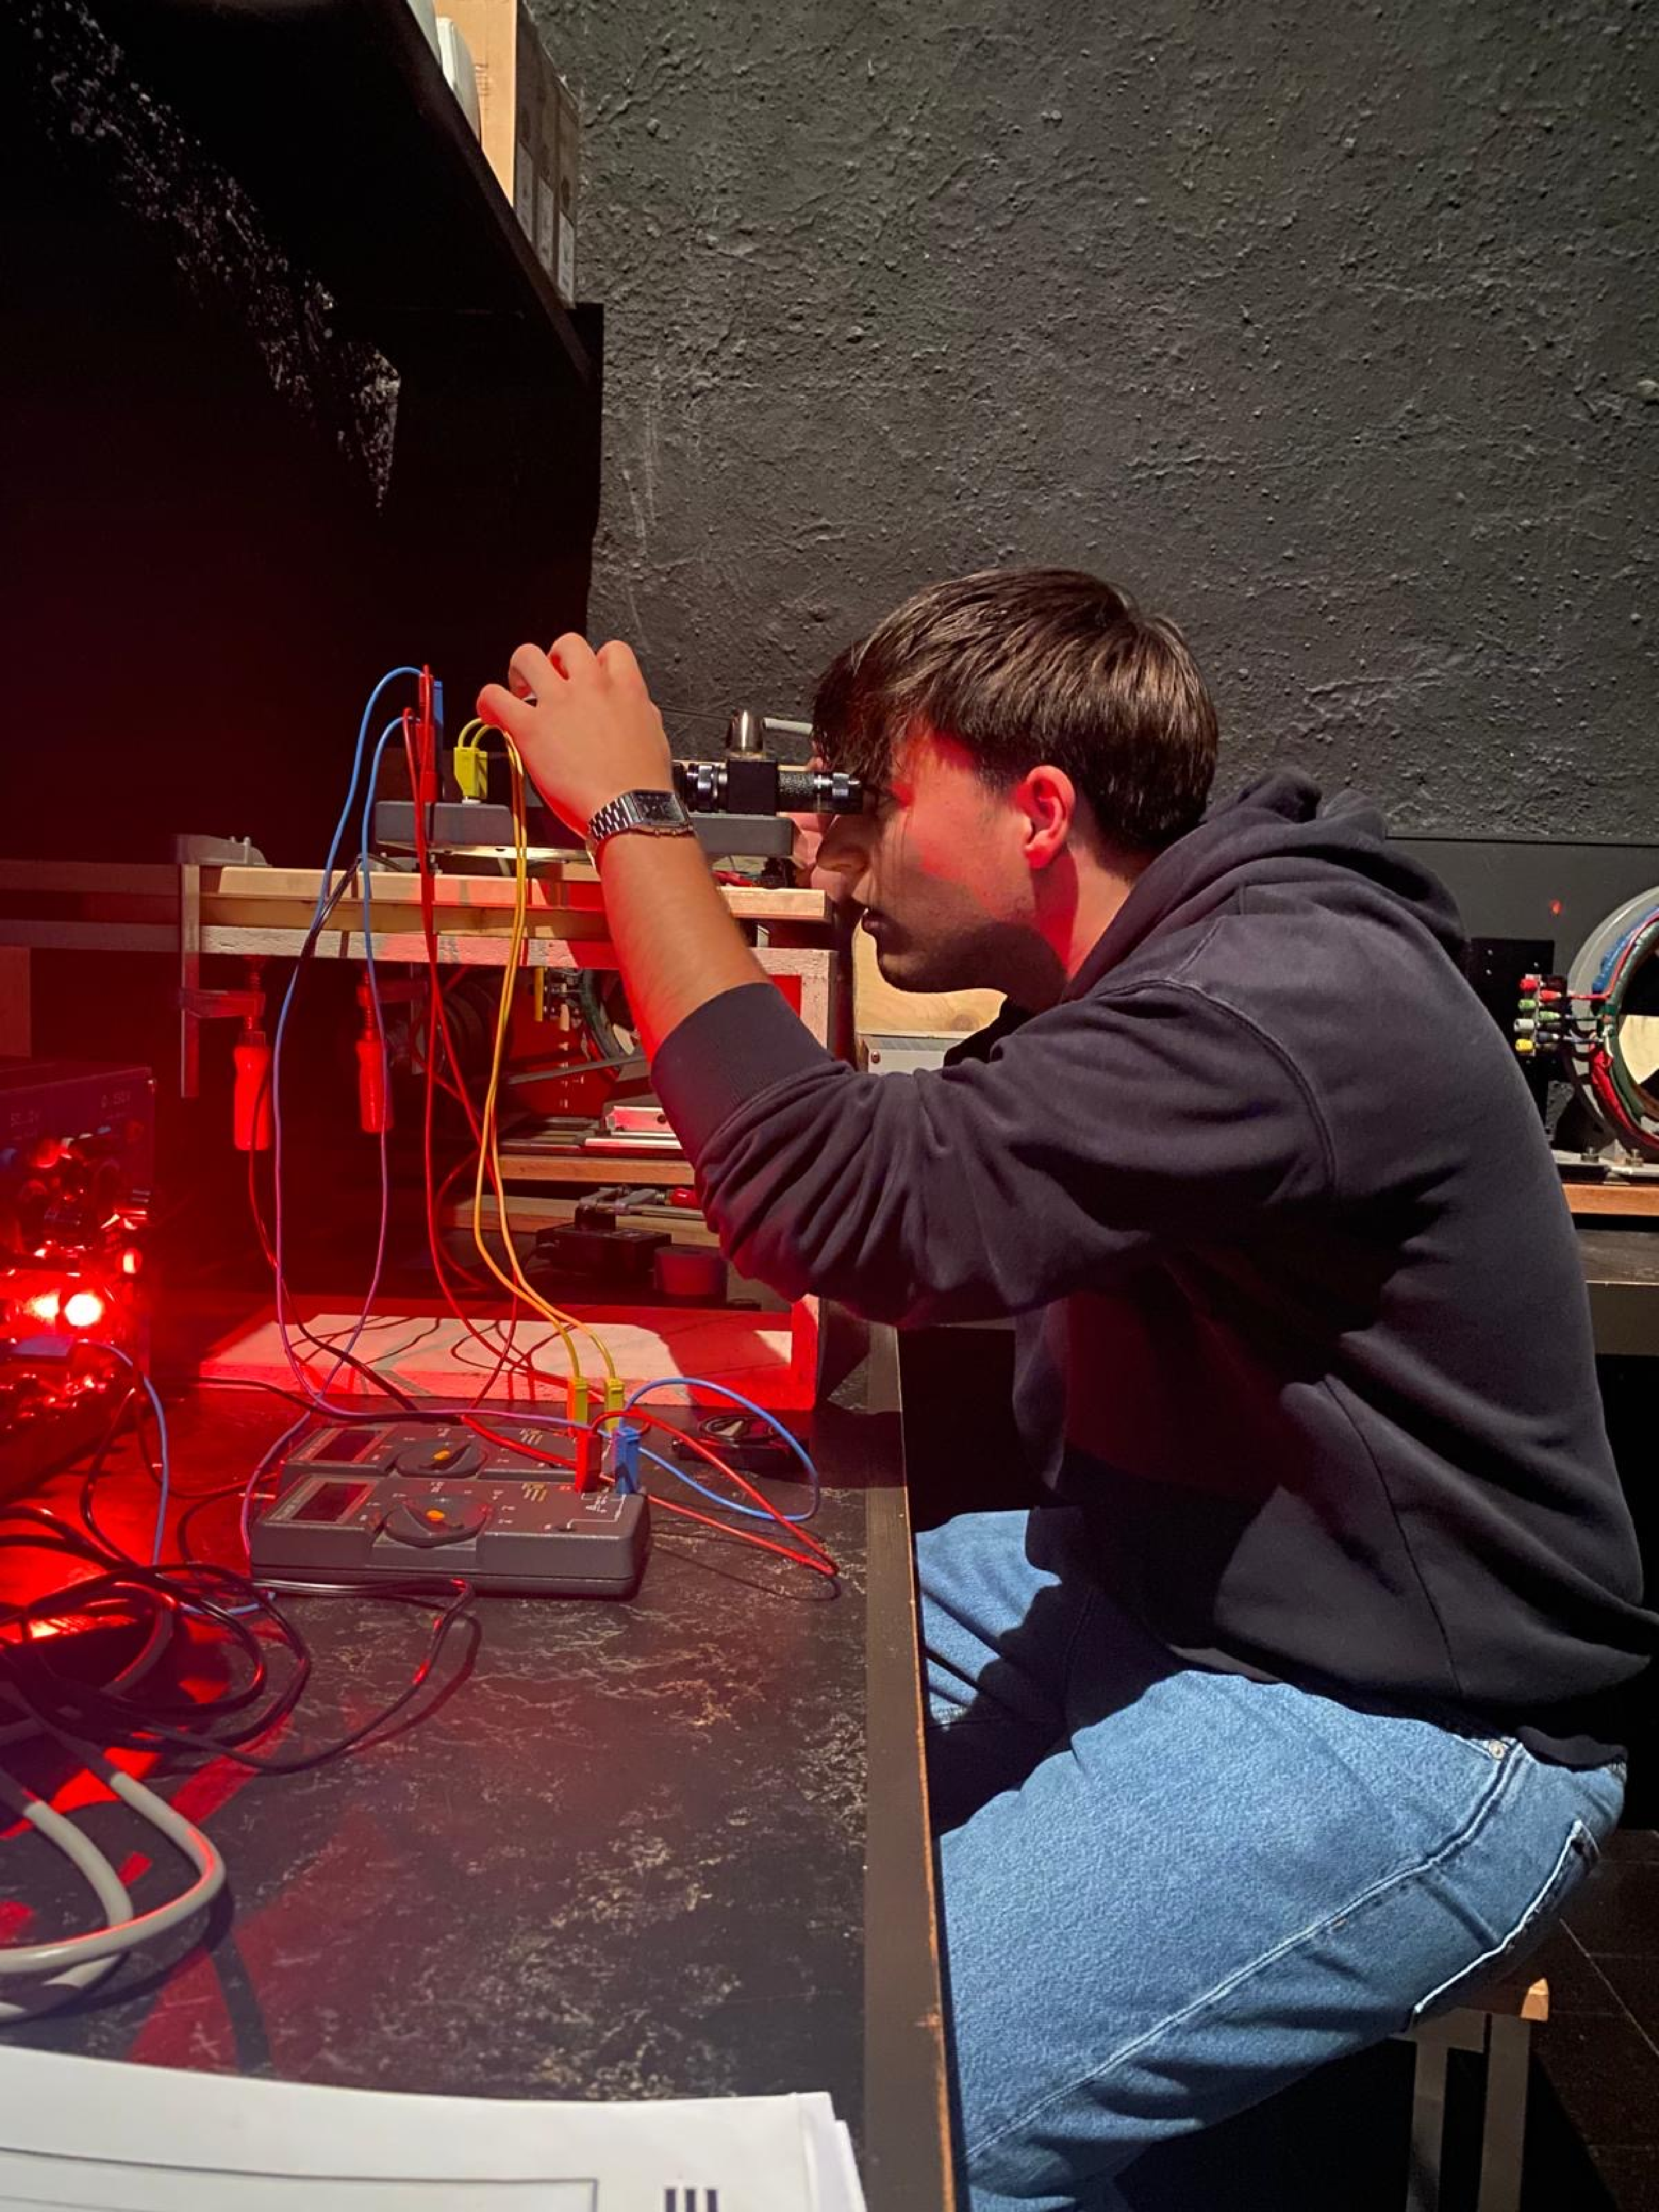
\includegraphics[scale=0.25]{bilder/pdf/bildExperimentieren.pdf}
	\caption{Bild während dem Experimentieren}
	\label{fig:experimentieren}
\end{figure}